\documentclass{article}
\usepackage[utf8]{inputenc}
\usepackage[spanish.mexico]{babel}
\usepackage[american voltages, american currents,siunitx]{circuitikz}


\title{Sistemas de Comunicaciones}
\author{Pablo Vivar Colina\\


}
%\date{Septiembre 2017}

\usepackage{natbib}
\usepackage{graphicx}

\begin{document}

\maketitle

\section{Prefijos del Sistema Internacional}

\begin{table}[h!]
\centering

\begin{tabular}{|c|c|c|c|c|c|}
\hline
1000n    & 10n   & Prefijo     & Símbolo      & Escala corta n 1​ & Escala larga n 1​       \\ \hline
10006    & 1018  & exa         & E            & Quintillón        & Trillón                 \\ \hline
10005    & 1015  & peta        & P            & Cuatrillón        & Mil billones            \\ \hline
10004    & 1012  & tera        & T            & Trillón           & Billón                  \\ \hline
10003    & 109   & giga        & G            & Billón            & Mil millones / Millardo \\ \hline
10002    & 106   & mega        & M            & Millón            & 1 000 000               \\ \hline
10001    & 103   & kilo        & k            & Mil / Millar      & 1 000                   \\ \hline
10002/3  & 102   & hecto       & h            & Cien / Centena    & 100                     \\ \hline
10001/3  & 101   & deca        & da           & Diez / Decena     & 10                      \\ \hline
10000    & 100   & Sin prefijo & Uno / Unidad & 1                 &                         \\ \hline
1000−1/3 & 10−1  & deci        & d            & Décimo            & 0.1                     \\ \hline
1000−2/3 & 10−2  & centi       & c            & Centésimo         & 0.01                    \\ \hline
1000−1   & 10−3  & mili        & m            & Milésimo          & 0.001                   \\ \hline
1000−2   & 10−6  & micro       & µ            & Millonésimo       & 0.000 001               \\ \hline
1000−3   & 10−9  & nano        & n            & Billonésimo       & Milmillonésimo          \\ \hline
1000−4   & 10−12 & pico        & p            & Trillonésimo      & Billonésimo             \\ \hline
1000−5   & 10−15 & femto       & f            & Cuatrillonésimo   & Milbillonésimo          \\ \hline
1000−6   & 10−18 & atto        & a            & Quintillonésimo   & Trillonésimo            \\ \hline
\end{tabular}
\caption{Tabla de prefijos \citep{PSI}}
\label{my-label}
\end{table}

\section{Elementos activos y pasivos en un circuito eléctrico}

\subsection{Elementos Pasivos}

Elementos pasivos son aquellos componentes de los circuitos, que disipan o almacenan energía eléctrica o magnética y constituyen por ello los receptores o cargas de un circuito. Estos elementos son modelos matemáticos lineales e ideales de los elementos físicos del circuito.\citep{EAP}\\

pueden presentar las siguientes propiedades:

\begin{enumerate}
    \item disipación de energía eléctrica (R: resistencia)
    \item almacenamiento de energía en campos magnéticos (L: coef. de autoinducción)
    \item almacenamiento de energía en campos eléctricos (C: capacidad).
\end{enumerate}
 
 Como ejemplo se encuentran la resistencia, inductancia y capacitancia.\citep{EAP}\\
 
 \subsection{Elementos Activos}
 
  Los componentes activos son aquellos que son capaces de excitar los circuitos o de realizar ganancias o control del mismo. Fundamentalmente son los generadores eléctricos y ciertos componentes semiconductores.\citep{EAP}\\
  
    Los generadores de corriente mantienen las características de la corriente entre sus bornes, independientemente de los elementos que componen el resto del circuito. Cuando esto no ocurre así se dice que se comporta como un generador real de corriente.\citep{EAP}\\


\section{Corriente alterna frente a la continua}

La razón del amplio uso de la corriente alterna viene determinada por su facilidad de transformación, cualidad de la que carece la corriente continua. En el caso de la corriente continua, la elevación de la tensión se logra conectando dínamos en serie, lo que no es muy práctico; al contrario, en corriente alterna se cuenta con un dispositivo, el transformador, que permite elevar la tensión de una forma eficiente.\citep{CA}\\

La energía eléctrica viene dada por el producto de la tensión, la intensidad y el tiempo. Dado que la sección de los conductores de las líneas de transporte de energía eléctrica depende de la intensidad, mediante un transformador se puede elevar la tensión hasta altos valores (alta tensión), disminuyendo en igual proporción la intensidad de corriente. Con esto la misma energía puede ser distribuida a largas distancias con bajas intensidades de corriente y, por tanto, con bajas pérdidas por causa del efecto Joule y otros efectos asociados al paso de corriente, tales como la histéresis o las corrientes de Foucault. Una vez en el punto de consumo o en sus cercanías, el voltaje puede ser de nuevo reducido para su uso industrial o doméstico y comercial de forma cómoda y segura.\citep{CA}\\


\section{Las matemáticas y la CA sinusoidal}

Algunos tipos de oscilaciones periódicas tienen el inconveniente de no tener definida su expresión matemática, por lo que no se puede operar analíticamente con ellas. Por el contrario, la oscilación sinusoidal no tiene esta indeterminación matemática y presenta las siguientes ventajas:\citep{CA}\\

\begin{itemize}
    \item La función seno está perfectamente definida mediante su expresión analítica y gráfica. Mediante la teoría de los números complejos se analizan con suma facilidad los circuitos de alterna.
    
    \item Las oscilaciones periódicas no sinusoidales se pueden descomponer en suma de una serie de oscilaciones sinusoidales de diferentes frecuencias que reciben el nombre de armónicos. Esto es una aplicación directa de las series de Fourier.
    
    \item Se pueden generar con facilidad y en magnitudes de valores elevados para facilitar el transporte de la energía eléctrica.
    
    \item Su transformación en otras oscilaciones de distinta magnitud se consigue con facilidad mediante la utilización de transformadores.
    
\end{itemize}

\subsection{Oscilación Senoidal}

Una señal senoidal o sinusoidal, $a(t)$, tensión, $v(t)$, o corriente, $i(t)$, se puede expresar matemáticamente según sus parámetros característicos (figura \ref{fig:ondaSenoidal}), como una función del tiempo por medio de la siguiente ecuación:\citep{CA}

\begin{equation}
    a(t)=A_0 \cdot \sin(\omega t + \beta)
\end{equation}
\begin{itemize}
    \item $A_0$ es la ''amplitud'' en [V] o [A] (también llamado ''valor máximo o de pico'')
    
    \item $\omega$  pulsación en radianes/segundo
    
    \item $t$ el tiempo en [s]
    
    \item $\beta$ el ángulo de fase inicial en radianes.
\end{itemize}


Dado que la velocidad angular es más interesante para matemáticos que para ingenieros, la fórmula anterior se suele expresar como:\citep{CA}\\

\begin{equation}
    a(t)=A_0 \cdot \sin(2 \pi f t + \beta)
\end{equation}


donde ''f'' es la frecuencia (Hz) y equivale a la inversa del período $f=\frac{1}{T}$. Los valores más empleados en la distribución son 50 Hz y 60 Hz.\citep{CA}


\begin{figure}[h!]
    \centering
    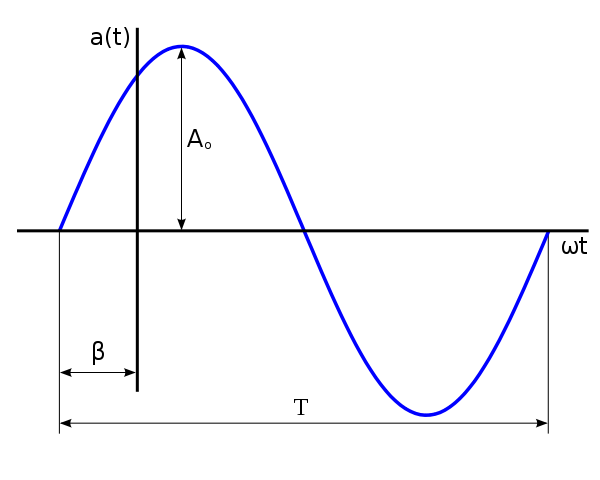
\includegraphics[scale=0.5]{Imagenes/600px-OndaSenoidal.png}
    \caption{Parámetros característicos de una oscilación sinusoidal.}
    \label{fig:ondaSenoidal}
\end{figure}

\section{Resistencia e Impedancia}

La impedancia (Z) es una medida de oposición que presenta un circuito a una corriente cuando se aplica una tensión. La impedancia extiende el concepto de resistencia a los circuitos de corriente alterna (CA), y posee tanto magnitud como fase, a diferencia de la resistencia, que sólo tiene magnitud.\\

\section{Circuito a resolver}

\begin{figure}[h!]
    \centering
   % \includegraphics{}
    \begin{circuitikz}
\draw

(-1,0)--(-1,-1)
(-1,-1) to[V,l=$28v$](-1,-2) 
 (-1,-2)--(-1,-3)
 
 (-1,-3)--(2,-3)
 
 (-1,0) to[R,l=$50 \Omega $](2,0)
 
 
 (2,-3)to[R,l=$5 \Omega$](2,0)
 
 (2,0)--(4,0)
 (2,-3)--(4,-3)
 
  (4,-3)to[R,l=$10 \Omega$](4,0)
 
 
;

%\draw[thick,arrows=->]
%(2.5,0)--(2.5,-1)
%;
 
\end{circuitikz}
    \caption{Circuito a resolver}
    \label{fig:circuito}
\end{figure}

%\subsection{Resultados}

Para resolver el circuito se hicieron equivalente los resistores de 5 y 10 $\Omegas$ para obtener el voltaje en esas ramas, así se pudo deducir la corriente en la rama del resistor de 50 $\Omega$ y el circuito equivalente, posterirmente se usaron las leyes de Kirchhoff para deducir los voltajes y las corrientes respectivamente.

\begin{table}[h!]
\centering

\begin{tabular}{|c|c|c|}
\hline
Componente & V {[}V{]} & I {[}A{]} \\ \hline
R 50       & 26.25     & 0.525     \\ \hline
R 10       & 1.75      & 0.173     \\ \hline
R 5        & 1.75      & 0.352     \\ \hline
V fuente   & 28        & 0.525     \\ \hline
\end{tabular}
\caption{Tabla de Resultados}
\label{tabla-resultados}

\end{table}

.\\[10cm]
\bibliographystyle{plain}
\bibliography{TareaPrefijos.bib}


\end{document}